\documentclass[conference]{IEEEtran}

\usepackage{amsmath,amssymb}
\usepackage{graphicx}
\usepackage{cite}
\usepackage{float}
\usepackage{stfloats}
\usepackage{hyperref}

\title{NTIRE 2026 Remote Sensing Infrared Image Super-Resolution Challenge Factsheet\\}

\author{Sulocha Yatageri$^{1,4}$, Saiprasad Meesiyawar$^{4}$, Nikhil Akalwadi$^{2,4}$, Ramesh Ashok Tabib$^{3,4}$, Uma Mudenagudi$^{3,4}$\\
{\normalsize \(^1\)Department of Computer Applications} {\normalsize \(^2\)School of Computer Science and Engineering} \\
{\normalsize \(^3\)Department of Electronics and Communication Engineering} {\normalsize \(^4\)Center for Visual Intelligence (CEVI)}\\
KLE Technological University, Hubballi, Karnataka, INDIA\\
[6pt]
\texttt{{\{01fe23bca107,}
\texttt{nikhil.akalwadi,}\\
\texttt{ramesh\_t, uma\}}
@kletech.ac.in}
\texttt{saiprasad@cevi.co.in}
}

\begin{document}

\maketitle

\section{Factsheet Information}

\subsection{Team details}

\begin{itemize}

\item \textbf{Team name}: KLETech-CEVI

\item \textbf{Team leader name}: Saiprasad Meesiyawar$^{4}$

\item \textbf{Team leader address, phone number, and email}:\\
Center for Visual Intelligence,\\
KLE Technological University, Hubballi\\
\textbf{Phone Number}: +91 9738924972\\
\textbf{Email}: saiprasad@cevi.co.in

\item \textbf{Rest of the team members}:
\begin{itemize}
\item Sulocha Yatageri$^{1,4}$
\item Nikhil Akalwadi$^{2,4}$
\item Ramesh Ashok Tabib$^{3,4}$
\item Uma Mudenagudi$^{3,4}$
\end{itemize}

\item \textbf{Team website URL}: \href{https://cevi.co.in}{https://cevi.co.in}

\item \textbf{Affiliation}:\\
$^1$Department of Computer Applications, KLE Technological University\\
$^2$Department of Computer Science Engineering, KLE Technological University\\
$^3$Department of Electronics and Communication Engineering, KLE Technological University\\
$^4$Center for Visual Intelligence (CEVI), KLE Technological University

\item \textbf{Affiliation of the team and/or team members with NTIRE 2026 sponsors:} NA

\item \textbf{User names and entries on the NTIRE 2026 competition platform:}\\saachi

\item \textbf{Best scoring entries during development phase:}\\Score: 51.453\\PSNR: 33.8246\\SSIM: 0.8814

\item \textbf{Link to the codes/executables of the solution(s):}
\href{https://github.com/CeviKle/NTIRE2026-KLETech-CEVI-RemoteSensing.git}{https://github.com/CeviKle/NTIRE2026-KLETech-CEVI-RemoteSensing.git}

\end{itemize}

\subsection{Method details}

Our proposed FreMamba method is designed for remote sensing infrared image super-resolution. Infrared remote sensing images often suffer from low spatial resolution due to sensor limitations, atmospheric effects, and acquisition constraints. This reduces the visibility of fine thermal structures, weak boundaries, and important scene details. To address this problem, we propose a Frequency-Assisted Vision State Space framework that combines global dependency modeling with local frequency-aware enhancement.

Given an input low-resolution infrared image $x$, the network first extracts shallow features using convolution layers:

\begin{equation}
F_{0} = Conv(x)
\end{equation}

where $F_{0}$ denotes the shallow feature representation extracted from the input image.

% ================= ARCHITECTURE FIGURE =================
\begin{figure*}[!t]
\centering
\includegraphics[width=0.96\textwidth]{architecture.png}
\caption{Overview of the proposed Frequency-Assisted Vision State Space architecture for remote sensing infrared image super-resolution. The low-resolution infrared image is first processed by a convolution layer for shallow feature extraction. The extracted features are then passed through multiple Frequency-assisted Mamba Groups (FMG), each containing Frequency-assisted Mamba Blocks (FMB). Inside each FMB, the global branch employs the Vision State Space Module (VSSM) to capture long-range dependencies, while the local branch uses the Frequency Selection Module (FSM) and Hybrid Gate Module (HGM) for frequency-aware refinement. The final feature representation is reconstructed into a high-resolution infrared image using convolution layers followed by PixelShuffle upsampling.}
\label{fig:architecture}
\end{figure*}

% ================= QUALITATIVE COMPARISON =================
\begin{figure*}[!t]
\centering
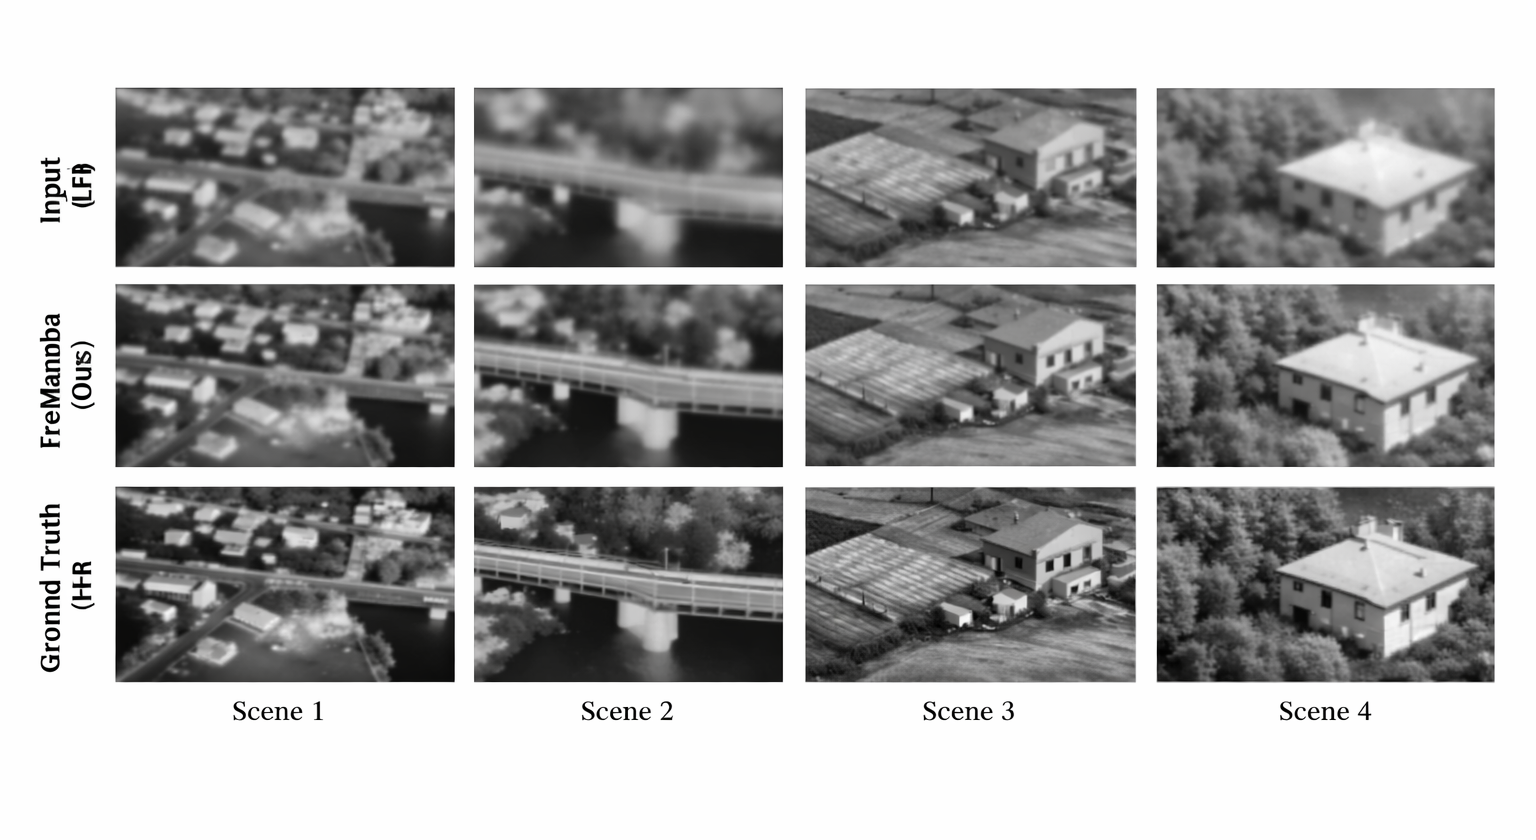
\includegraphics[width=0.96\textwidth]{quality_comparison.png}
\caption{Qualitative comparison of the proposed FreMamba for Remote Sensing Infrared Image Super-Resolution (4$\times$). The first row shows the low-resolution infrared input images, while the second row shows the reconstructed high-resolution outputs generated by FreMamba. Zoomed regions demonstrate that the proposed method effectively restores fine structural details and suppresses noise.}
\label{fig:qualitative}
\end{figure*}

The extracted shallow features are then processed through multiple Frequency-assisted Mamba Groups (FMG). Each FMG contains several Frequency-assisted Mamba Blocks (FMB), which are designed to capture both global and local feature interactions.

\begin{equation}
F_{i} = FMG_{i}(F_{i-1})
\end{equation}

where $F_i$ denotes the output feature map of the $i^{th}$ FMG.

Each Frequency-assisted Mamba Block consists of two complementary branches.

The global branch captures long-range spatial dependencies using the Vision State Space Module (VSSM):

\begin{equation}
F_{g} = VSSM(LN(F))
\end{equation}

The local branch enhances high-frequency information through the Frequency Selection Module (FSM) and Hybrid Gate Module (HGM):

\begin{equation}
F_{l} = FSM(HGM(LN(F)))
\end{equation}

The outputs of the global and local branches are fused through residual aggregation. The reconstructed super-resolved image is obtained using convolution and PixelShuffle upsampling:

\begin{equation}
\hat{y} = PixelShuffle(Conv(F_{fusion}))
\end{equation}

We optimize the network using a weighted combination of losses:

\begin{equation}
L_{FreMamba} = (\alpha L_{MSE}) + (\beta L_{Charb}) + (\gamma L_{SSIM})
\end{equation}

Mean Squared Error loss:

\begin{equation}
L_{MSE} = \frac{1}{N}\sum (I_{SR} - I_{HR})^{2}
\end{equation}

Charbonnier loss:

\begin{equation}
L_{Charb} = \frac{1}{N}\sum \sqrt{(I_{SR}-I_{HR})^{2}+\epsilon^{2}}
\end{equation}

SSIM loss:

\begin{equation}
L_{SSIM} = 1 - SSIM(I_{SR},I_{HR})
\end{equation}

\begin{itemize}

\item \textbf{Training strategy}

We train the proposed methodology using the dataset provided for the NTIRE 2026 Remote Sensing Infrared Image Super-Resolution Challenge. The implementation is performed using Python and PyTorch. Training is conducted on $64\times64$ patches with a batch size of 4 using the Adam optimizer. The model is trained for 300 epochs with a learning rate of 0.0001.

\item \textbf{Total method complexity}

\begin{itemize}
\item Number of parameters:
\item FLOPs:
\item GPU memory consumption:
\item Total training time:
\item Inference time / image:
\end{itemize}

\item \textbf{External models used}

The proposed architecture is based on the Frequency-Assisted Vision State Space Model (FreMamba). Pre-trained checkpoints may optionally be used for initialization before fine-tuning.

\item \textbf{Additional data used}

No additional datasets were used beyond the NTIRE provided training and validation data.

\item \textbf{Training description}

Training is performed using paired low-resolution and high-resolution infrared images. Data augmentation techniques such as random cropping, flipping, and rotation are applied during training.

\item \textbf{Testing description}

During testing, the trained model generates super-resolved infrared images from the validation and test datasets. Inference is performed on a single GPU.

\item \textbf{Quantitative and qualitative advantages}

The proposed framework achieves strong PSNR and SSIM performance. Qualitatively, the model reconstructs sharper thermal boundaries and improved high-frequency structures while preserving thermal consistency. The qualitative results are illustrated in Fig.~\ref{fig:qualitative}.

\end{itemize}

\section{Other details}

\begin{itemize}

\item \textbf{Planned submission of solution description paper at NTIRE 2026 workshop}

\item \textbf{Other comments}

The main challenges encountered included dataset organization, dataloader stabilization, checkpoint selection, and tuning loss functions to improve PSNR performance.

\end{itemize}
\section{References}
\vspace{-0.5cm}  % adjust this value if needed
\renewcommand{\refname}{} % removes automatic "References" heading
\begin{thebibliography}{00}

\bibitem{fremamba}
K. Liu, H. Yue, Z. Lin, Z. Chen, J. Wang, J. Gong, R. Timofte, and Y. Zhang,
``Frequency-Assisted Mamba for Remote Sensing Image Super-Resolution,''
in \textit{Proc. NTIRE Workshop}, 2026.

\bibitem{mamba}
A. Gu and T. Dao,
``Mamba: Linear-Time Sequence Modeling with Selective State Spaces,''
in \textit{Proc. International Conference on Learning Representations (ICLR)}, 2024.


\bibitem{edsr}
B. Lim, S. Son, H. Kim, S. Nah, and K. M. Lee,
``Enhanced Deep Residual Networks for Single Image Super-Resolution,''
in \textit{Proc. IEEE Conference on Computer Vision and Pattern Recognition Workshops (CVPRW)}, 2017.


\end{thebibliography}

\end{document}